\documentclass[12pt]{article}
%%---------------------------------------------------------------------
% packages
% geometry
\usepackage{geometry}
% font
\usepackage{fontspec}
\defaultfontfeatures{Mapping=tex-text}  %%如果没有它,会有一些 tex 特殊字符无法正常使用,比如连字符。
\usepackage{xunicode,xltxtra}
\usepackage[BoldFont,SlantFont,CJKnumber,CJKchecksingle]{xeCJK}  % \CJKnumber{12345}: 一万二千三百四十五
\usepackage{CJKfntef}  %%实现对汉字加点、下划线等。
\usepackage{pifont}  % \ding{}
% math
\usepackage{amsmath,amsfonts,amssymb}
% color
\usepackage{color}
\usepackage{xcolor}
\definecolor{EYE}{RGB}{199,237,204}
\definecolor{FLY}{RGB}{128,0,128}
\definecolor{ZHY}{RGB}{139,0,255}
% graphics
\usepackage[americaninductors,europeanresistors]{circuitikz}
\usepackage{tikz}
\usetikzlibrary{positioning,arrows,shadows,shapes,calc,mindmap,trees,backgrounds}  % placements=positioning
\usepackage{graphicx}  % \includegraphics[]{}
\usepackage{subfigure}  %%图形或表格并排排列
% table
\usepackage{colortbl,dcolumn}  %% 彩色表格
\usepackage{multirow}
\usepackage{multicol}
\usepackage{booktabs}
% code
\usepackage{fancyvrb}
\usepackage{listings}
% title
\usepackage{titlesec}
% head/foot
\usepackage{fancyhdr}
% ref
\usepackage{hyperref}
% pagecolor
\usepackage[pagecolor={EYE}]{pagecolor}
% tightly-packed lists
\usepackage{mdwlist}

\usepackage{styles/iplouccfg}
\usepackage{styles/zhfontcfg}
\usepackage{styles/iplouclistings}

%%---------------------------------------------------------------------
% settings
% geometry
\geometry{left=2cm,right=1cm,top=2cm,bottom=2cm}  %设置 上、左、下、右 页边距
\linespread{1.5} %行间距
% font
\setCJKmainfont{Adobe Kaiti Std}
%\setmainfont[BoldFont=Adobe Garamond Pro Bold]{Apple Garamond}  % 英文字体
%\setmainfont[BoldFont=Adobe Garamond Pro Bold,SmallCapsFont=Apple Garamond,SmallCapsFeatures={Scale=0.7}]{Apple Garamond}  %%苹果字体没有SmallCaps
\setCJKmonofont{Adobe Fangsong Std}
% graphics
\graphicspath{{figures/}}
\tikzset{
    % Define standard arrow tip
    >=stealth',
    % Define style for boxes
    punkt/.style={
           rectangle,
           rounded corners,
           draw=black, very thick,
           text width=6.5em,
           minimum height=2em,
           text centered},
    % Define arrow style
    pil/.style={
           ->,
           thick,
           shorten <=2pt,
           shorten >=2pt,},
    % Define style for FlyZhyBall
    FlyZhyBall/.style={
      circle,
      minimum size=6mm,
      inner sep=0.5pt,
      ball color=red!50!blue,
      text=white,},
    % Define style for FlyZhyRectangle
    FlyZhyRectangle/.style={
      rectangle,
      rounded corners,
      minimum size=6mm,
      ball color=red!50!blue,
      text=white,},
    % Define style for zhyfly
    zhyfly/.style={
      rectangle,
      rounded corners,
      minimum size=6mm,
      ball color=red!25!blue,
      text=white,},
    % Define style for new rectangle
    nrectangle/.style={
      rectangle,
      draw=#1!50,
      fill=#1!20,
      minimum size=5mm,
      inner sep=0.1pt,}
}
\ctikzset{
  bipoles/length=.8cm
}
% code
\lstnewenvironment{VHDLcode}[1][]{%
  \lstset{
    basicstyle=\footnotesize\ttfamily\color{black},%
    columns=flexible,%
    framexleftmargin=.7mm,frame=shadowbox,%
    rulesepcolor=\color{blue},%
%    frame=single,%
    backgroundcolor=\color{yellow!20},%
    xleftmargin=1.2\fboxsep,%
    xrightmargin=.7\fboxsep,%
    numbers=left,numberstyle=\tiny\color{blue},%
    numberblanklines=false,numbersep=7pt,%
    language=VHDL%
    }\lstset{#1}}{}
\lstnewenvironment{VHDLmiddle}[1][]{%
  \lstset{
    basicstyle=\scriptsize\ttfamily\color{black},%
    columns=flexible,%
    framexleftmargin=.7mm,frame=shadowbox,%
    rulesepcolor=\color{blue},%
%    frame=single,%
    backgroundcolor=\color{yellow!20},%
    xleftmargin=1.2\fboxsep,%
    xrightmargin=.7\fboxsep,%
    numbers=left,numberstyle=\tiny\color{blue},%
    numberblanklines=false,numbersep=7pt,%
    language=VHDL%
    }\lstset{#1}}{}
\lstnewenvironment{VHDLsmall}[1][]{%
  \lstset{
    basicstyle=\tiny\ttfamily\color{black},%
    columns=flexible,%
    framexleftmargin=.7mm,frame=shadowbox,%
    rulesepcolor=\color{blue},%
%    frame=single,%
    backgroundcolor=\color{yellow!20},%
    xleftmargin=1.2\fboxsep,%
    xrightmargin=.7\fboxsep,%
    numbers=left,numberstyle=\tiny\color{blue},%
    numberblanklines=false,numbersep=7pt,%
    language=VHDL%
    }\lstset{#1}}{}
% pdf
\hypersetup{pdfpagemode=FullScreen,%
            pdfauthor={Haiyong Zheng},%
            pdftitle={Title},%
            CJKbookmarks=true,%
            bookmarksnumbered=true,%
            bookmarksopen=false,%
            plainpages=false,%
            colorlinks=true,%
            citecolor=green,%
            filecolor=magenta,%
            linkcolor=cyan,%red(default)
            urlcolor=cyan}
% section
%http://tex.stackexchange.com/questions/34288/how-to-place-a-shaded-box-around-a-section-label-and-name
\newcommand\titlebar{%
\tikz[baseline,trim left=3.1cm,trim right=3cm] {
    \fill [cyan!25] (2.5cm,-1ex) rectangle (\textwidth+3.1cm,2.5ex);
    \node [
        fill=cyan!60!white,
        anchor= base east,
        rounded rectangle,
        minimum height=3.5ex] at (3cm,0) {
        \textbf{\thesection.}
    };
}%
}
\titleformat{\section}{\Large\bf\color{blue}}{\titlebar}{0.1cm}{}
% head/foot
\setlength{\headheight}{15pt}
\pagestyle{fancy}
\fancyhf{}
%\lhead{\color{black!50!green}2014年秋季学期}
\chead{\color{black!50!green}图像特征}
%\rhead{\color{black!50!green}通信电子电路}
\lfoot{\color{blue!50!green}朱亚菲}
\cfoot{\color{blue!50!green}\href{http://vision.ouc.edu.cn/~zhenghaiyong}{CVBIOUC}}
\rfoot{\color{blue!50!green}$\cdot$\ \thepage\ $\cdot$}
\renewcommand{\headrulewidth}{0.4pt}
\renewcommand{\footrulewidth}{0.4pt}


%%---------------------------------------------------------------------
\begin{document}
%%---------------------------------------------------------------------
%%---------------------------------------------------------------------
% \titlepage
\title{\vspace{-2em}图像特征\vspace{-0.7em}}
\author{朱亚菲}
\date{\vspace{-0.7em}2015年1月\vspace{-0.7em}}
%%---------------------------------------------------------------------
\maketitle\thispagestyle{fancy}
%%---------------------------------------------------------------------
\maketitle
\tableofcontents 


\section{引言}

\section{局部图像特征描述}

\url{http://www.sigvc.org/bbs/thread-165-1-1.html}

局部特征,顾名思义就是一些局部才会出现的特征,

局部图像特征描述的核心问题是不变性(鲁棒性)和可区分性。由于使用局部图像特征描述子的时候,通常是为了鲁棒地处理各种图像变换的情况。因此,在构建/设计特征描述子的时候,不变性问题就是首先需要考虑的问题。

\section{全局图像特征描述}

如果用户对整个图像的整体感兴趣,而不是对前景本身感兴趣的话,用全局特征来描述图像是比较合适的。但是无法分辨出前景和背景却是全局特征本身就有的劣势,特别是在关注的对象受到遮挡等影响的时候,全局特征很有可能就被破坏掉了。所以全局特征一般被用到图像检索、图像分类等领域。

\subsection{图像直方图}

图像直方图是指统计图像中像素的灰度/颜色得到的图像灰度/颜色频数图。直方图由于其计算代价较小,且具有图像平移、旋转、缩放不变性等优点,广泛应用于图像处理的各个领域。Swain和Ballard最先提出了使用颜色直方图作为图像颜色特征的表示方法。

传统颜色直方图描述方法存在以下问题:

1)颜色特征维数高。以8bit的RGB颜色空间为例,全颜色数为$256 \times 256 \times 256$种颜色,如果以全颜色数统计直方图,则存储空间和计算复杂度都较大。

2)颜色特征受光照影响。即对于两幅颜色分布很类似却因光照不同导致亮度差异大的图像,理论上,其颜色直方图应相似,但实际传统颜色直方图却不相似。

3)不能表达相近颜色间相关性,即传统颜色直方图的颜色间完全独立,不能反映相近颜色间的关联。理论上,对于发生较小颜色偏移的两幅图像间应相似。如,一幅完全红色的图像与另一幅完全浅红色的图像间相似度较高。而实际传统颜色直方图却不相似。

4)丢失空间位置信息,因此该特征无法区分颜色相同而空间分布不同的两幅图像。

得到图像颜色特征后 需要定义颜色特征的相似度量公式,以表示两幅图像间颜色的相似性。不同的相似性度量公式对实际应用结果可能影响很大。因此需要研究如何选择或设计合适的相似性度量算法。

显著性Models中,CB、DRFI、HC/RC、HDCT方法都用到了颜色直方图。在显著性检测中,由于关注的是显著目标,并且用到中央-周围对比,因此用到的应该都是局部特征。

DRFI方法中关于图像RGB空间的颜色直方图代码如下:

\lstinputlisting{RGBhistogram.m}

首先对图像($300 \times 400$)的颜色空间进行量化,将颜色空间划分为若干个小的颜色区间,即直方图的bin,例如将每个颜色通道量化为只有16个不同值,此时$bin = 16 \times 16 \times 16$,然后计算矩阵$Q$($300 \times 400$),用其中的值代表颜色,而不是用$(r, g, b)$向量表示颜色,$Q$中有多少个不同值表示图像中有多少种颜色。结果如图~\ref{fig: RGBhistogram}。

\begin{figure}
  \centering 
  \subfigure[]{ 
    \label{fig: RGBhistogram: a} %% label for first subfigure 
    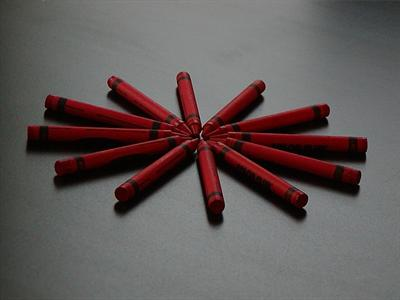
\includegraphics[width=0.45\textwidth]{example1.jpg}} 
  \subfigure[]{ 
    \label{fig: RGBhistogram: b} %% label for second subfigure 
    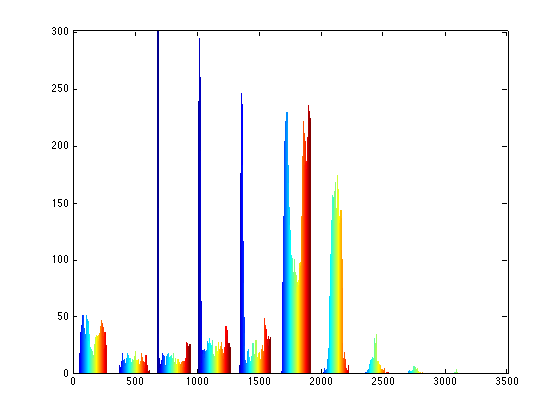
\includegraphics[width=0.45\textwidth]{RGBhistogram1.png}} 
  \caption{RGB空间的颜色直方图}
  \label{fig: RGBhistogram} %% label for entire figure 
\end{figure}

颜色空间

1)RGB颜色空间

RGB颜色空间是常用的表示彩色图像的一种颜色空间,它是以红、绿、蓝三种颜色为基础,亦称为“三原色”。所谓的“原色”是一种生物学概念,是根据人眼对光线感知的生理作用来定义的。每一种颜色按亮度进行分类,分成256个等级。不同比例的红、绿、蓝叠加,能产生丰富的颜色。例如,等比例的三原色进行相加可以产生白色,红色与绿色相加产生黄色。可见,RGB空间属于“叠加型”原色系统,因此把RGB颜色空间作为最基础的颜色空间,通过对RGB的非线性或线性变换可以获得其它的颜色空间。

2)CIELAB颜色空间

在许多文献中,CIELAB颜色空间也称CIE 1976 L*a*b(简写为CIE L*a*b)颜色空间。CIELAB颜色系统是使用最广泛的物体颜色度量方法,并作为度量颜色的国际标准。CIE 1976 L*a*b颜色空间是CIE 1931 XYZ颜色空间的一种数学变换的结果。

CIE 1976 L*a*b颜色空间和CIE 1931 XYZ颜色空间的相同之处是,它们都使用相同的基本原理,即颜色是光、物体和观察者组合的结果,三种基色值是用CIE定义的光、物体和观察者的数据进行计算得到的。

CIELAB系统使用的坐标叫做对色坐标(opponent color coordinate),使用对色坐标的想法来自这样的概念:颜色不能同时是红和绿,或者同时是黄和蓝,但颜色可以被认为是红和黄、红和蓝、绿和黄以及绿和蓝的组合。CIELAB使用L*, a*和b*坐标轴定义CIE颜色空间。其中,L*值代表光亮度,其值从0(黑色)~100(白色)。a*和b*代表色度坐标,其中a*代表红-绿轴,b*代表黄-蓝轴,它们的值从0~10。$a*=b*=0$表示无色,因此L*就代表从黑到白的比例系数。

































\end{document}